\documentclass[../NormeProgetto.tex]{subfiles}

\begin{document}
\section{Processi di supporto}
\subsection{Documentazione}
In questa sezione sono indicati gli standard riguardanti la struttura e la stesura dei documenti prodotti.
	\subsubsection{Struttura dei documenti}
		Ogni documento è realizzato a partire da una struttura prestabilita che dovrà essere uguale per tutti i documenti ufficiali ad eccezione dei verbali:
		\begin{enumerate}
			\item frontespizio;
			\item informazione sul documento;
			\item diario delle modifiche;
			\item indice delle sezioni;
			\item indice delle tabelle;
			\item indice delle figure;
			\item introduzione;
			\item contenuto.
		\end{enumerate}
		L'ordine di ognuna delle sezioni è fissato. La numerazione delle prime pagine sarà quella romana, mentre dall'introduzione fino alla fine del documento quella araba.

		\paragraph{Frontespizio}
			Questa sezione deve trovarsi nella prima pagina di ogni documento e contiene:
			\begin{enumerate}
				\item informazioni sul gruppo:
					\begin{enumerate}[a.]
						\item nome;
						\item logo;
						\item email.
					\end{enumerate}
				\item informazioni sul progetto:
					\begin{enumerate}[a.]
						\item nome progetto;
						\item nome azienda proponente.
					\end{enumerate}
				\item informazioni sul documento:
					\begin{enumerate}[a.]
						\item nome;
						\item versione.
					\end{enumerate}
			\end{enumerate}

		\paragraph{Informazioni sul documento}
			In questa sezione vengono indicate le principale informazioni riguardanti il documento quali:
			\begin{enumerate}
				\item versione;
				\item data di redazione;
				\item cognome e nome di coloro che hanno redatto il documento (in ordine alfabetico);
				\item cognome e nome di coloro che hanno verificato il documento (in ordine alfabetico);
				\item ambito d'uso del documento (interno oppure esterno);
				\item cognome e nome di coloro ai quali è destinato il documento (in ordine alfabetico).
			\end{enumerate}

		\paragraph{Diario delle modifiche}
			Questa sezione descrive, attraverso l'utilizzo di una tabella, le modifiche che sono state apportate al documento. Ogni riga della tabella corrisponde ad una modifica effettua al documento. La struttura della riga della tabella è la seguente:
			\begin{enumerate}
				\item versione del documento;
				\item data della modifica;
				\item cognome e nome dell'autore della modifica;
				\item ruolo dell'autore della modifica nel momento in cui essa è avvenuta;
				\item descrizione delle modifiche apportate.
			\end{enumerate}

			Le righe della tabella sono ordinate a partire dalla data dell'ultima modifica effettuata, in ordine cronologico inverso.

		\paragraph{Indice delle sezioni}
			L'indice delle sezioni contiene l'indice di tutti gli argomenti trattati all'interno del documento. La sua struttura è la seguente:

			\begin{enumerate}
				\item titolo dell'argomento trattato;
				\item numero di pagina.
			\end{enumerate}

		\paragraph{Indice delle tabelle}
			Questa sezione contiene l'indice delle tabelle. Per ogni tabella deve essere specificato:

			\begin{enumerate}
				\item titolo della tabella;
				\item numero di pagina di riferimento.
			\end{enumerate}

			Nel caso in cui non siano presenti tabelle all'interno del documento, è possibile omettere questa sezione.

		\paragraph{Indice delle figure}
			In questa sezione sono riportate tutte le figure presenti all'interno del documento. Per ogni figura deve essere specificato:
			\begin{itemize}
				\item nome figura;
				\item pagina di riferimento della figura.
			\end{itemize}
			Nel caso in cui non siano presenti figure all'interno del documento, è possibile omettere questa sezione.

		\paragraph{Introduzione}
			Questa sezione deve riportare le seguenti informazioni:
			\begin{enumerate}
				\item scopo del documento;
				\item glossario;
				\item riferimenti utili:
				\begin{enumerate}[a.]
					\item riferimenti normativi;
					\item riferimenti informativi.
				\end{enumerate}
			\end{enumerate}

		\paragraph{Contenuto}
			Questa sezione contiene il contenuto del documento. Anch'esso deve essere propriamente diviso in sezioni e sottosezioni.
	
	\subsubsection{Norme tipografiche} \label{sec:Norme tipografiche}
		\paragraph{Formattazione generale}
			\subparagraph{Testatine}
				Ogni pagina di un documento, fatta eccezione per il frontespizio, deve contenere la testina. Essa è composta da:
				\begin{itemize}
					\item logo del gruppo, posizionato in alto a sinistra;
					\item nome del documento, posizionato in alto a destra.
				\end{itemize}
			\subparagraph{Piè pagina}
				Ogni pagina di un documento, deve contenere il piè pagina. Esso contiene:
				\begin{itemize}
					\item numero della pagina, posizionato al centro.
				\end{itemize}
			\subparagraph{Orfani e vedove}
				Si considerano vedova, la riga di un paragrafo che inizia alla fine di una pagina, mentre si considera orfana, la riga di un paragrafo che finisce all'inizio di una pagina. I documenti dovranno essere redatti cercando di evitare il più possibile queste due tipologie di righe poiché risultano poco gradevoli. 
		\paragraph{Caratteri}
			
			\subparagraph{Virgolette}
				\begin{itemize}
					\item \textbf{Virgolette alte singole ` ' :} devono essere utilizzate per racchiudere un singolo carattere;
					\item \textbf{Virgolette alte doppie `` '' :} devono essere utilizzate per racchiudere:
					\begin{itemize}
						\item nomi di file;
						\item comandi;
						\item collegamenti a sezioni interne dello stesso documento;
						\item parole a cui è stato dato un significato particolare;
						\item parole a cui è stato dato un senso diverso da quello originale.
					\end{itemize}
					\item \textbf{Virgolette basse `<<' `>>' :} devono essere utilizzate per racchiudere citazioni.
				\end{itemize}
				Non sono ammessi ulteriori casi d'uso per le virgolette.
			
			\subparagraph{Parentesi}
				\begin{itemize}
					\item \textbf{Tonde:} possono essere utilizzate per descrivere esempi, per fornire dei sinonimi oppure per dare delle precisazioni. Sono le uniche parentesi ammesse all'interno di una frase.
					\item \textbf{Quadre:} possono rappresentare uno standard ISO oppure uno stato relativo ad un ticket\g. 
				\end{itemize}

			
			\subparagraph{Punteggiatura}
				La punteggiatura  deve essere sempre utilizzata attentamente per cercare di rendere il discorso il più chiaro e coeso possibile. Non sono ammesse spaziature prima dell'utilizzo di un carattere di punteggiatura. L'utilizzo del punto è necessario per indicare la fine di un concetto e poter iniziarne un altro.
			
			\subparagraph{Numeri}
				I numeri all'interno dei documenti devono essere formattati seguendo lo standard [SI/ISO 31-0]. Esso prevede che la parte frazionaria sia separata da quella decimale utilizzando la virgola. I numeri la cui parte intera supera le tre cifre, devono essere scritti raggruppando in gruppi di tre le cifre di cui è composta la parte intera, partendo dalla cifra meno significativa e separandoli con uno spazio unificatore.
			
		\paragraph{Stile del testo}

			\subparagraph{Corsivo}
				Il corsivo va utilizzato per riportare le seguenti informazioni:
				\begin{itemize}
					\item nome di un documento;
					\item nome di un ruolo;
					\item percorsi di cartelle.
				\end{itemize}						
			
			\subparagraph{Grassetto}
				Il grassetto va utilizzato per riportare le seguenti informazioni:
				\begin{itemize}
					\item titoli;
					\item parole su cui è utile focalizzare l'attenzione del lettore all'interno di un argomento;
					\item parole chiave all'interno di elenchi.
				\end{itemize}						
			
			\subparagraph{Sottolineato}
				La sottolineatura è indicata qualora si voglia evidenziare l'importanza di una parola all'interno di una frase.					
			
			\subparagraph{Monospace}
				Lo stile Monospace\g\ va applicato nel caso in cui si vogliano riportare all'interno di un documento	comandi oppure parti di codice.
			
			\subparagraph{Glossario}\label{sec:Formattazione termini nel glossario}
				Questo stile va applicato per tutte le parole che hanno una corrispondenza all'interno del glossario. Ogni parola presente nel glossario deve essere seguita da un pedice contente il carattere `g' scritto in corsivo. Non si applica questa regola nei casi in cui la parola compaia all'interno di titoli, percorsi, nomi di cartelle, comandi o parti di codice.
			
		\paragraph{Composizione del testo}
			\subparagraph{Elenchi}
				Le norme che regolano un elenco sono le seguenti:
				\begin{itemize}
					\item la prima parola di un elenco deve essere maiuscola, fatta eccezione nel caso in cui l'elenco inizi con il carattere `:';
					\item ogni elemento dell'elenco, tranne l'ultimo, deve terminare con il carattere `;'. È fatta eccezione nel caso in cui l'elemento sia composto da molte frasi, allora è permesso il `.';
					\item l'ultimo elemento di un elenco deve sempre terminare con il carattere `.'.
				\end{itemize}
				È necessario usare elenchi numerati quando l'ordine degli elementi è rilevante. Per gli elenchi numerati valgono le seguenti regole:
				\begin{itemize}
					\item nel primo livello si usano numeri interni a partire da uno;
					\item nel secondo livello si usano lettere dell'alfabeto a partire. dalla `a'.
				\end{itemize}
				Gli elenchi puntati servono per descrivere elementi di cui non è importante l'ordine espositivo. Essi seguono le seguenti regole:
				\begin{itemize}
					\item nel primo livello bisogna utilizzare cerchi neri pieni;
					\item nel secondo livello trattini neri.
				\end{itemize}
			
			
			\subparagraph{Descrizioni}
				Nel caso in cui si voglia strutturare la descrizione di qualcosa nella forma di elenco è necessario utilizzare il costrutto \LaTeX\ \texttt{ \textbackslash begin$\left\{description\right\}$ \textbackslash item[elemento] \textbackslash end$\left\{description\right\}$}. All'interno delle parentesi quadre viene inserito il nome dell'elemento che si vuole descrivere mentre, dopo di esse, la sua descrizione.					
			
			\subparagraph{Note a piè pagina}
				Le note a piè pagina seguono le seguenti regole:
				\begin{itemize}
					\item la loro numerazione è progressiva all'interno di tutto il documento;
					\item devono essere scritte una volta sola;
					\item il primo carattere di ogni nota deve essere maiuscolo. Fanno eccezione i casi in cui la parola sia un acronimo. In questo caso bisogna seguire le regole di formattazione di tale acronimo.
				\end{itemize}
			
		\paragraph{Formati}
			\subparagraph{Date}
				La formattazione delle date segue lo standard [ISO 8601]. Tale standard prevede che una data sia scritta secondo il seguente formalismo: AAAA-MM-GG. Questa rappresentazione va letta nel seguente modo:
				\begin{itemize}
					\item AAAA: numero a quattro cifre che rappresenta l'anno;
					\item MM: numero a due cifre che rappresenta il mese;
					\item GG: numero a due cifre che rappresenta il giorno.
				\end{itemize}
				Nei casi in cui risulti possibile esprimere i mesi o giorni omettendo una cifra, è necessario anteporre uno zero davanti a tale cifra. Per velocizzare la scrittura delle date è stato creato il comando \LaTeX\ \texttt{\textbackslash frmdate\{giorno\}\{mese\}\{anno\}}.
			
			\subparagraph{Orari}
				La formattazione degli orari segue lo standard [ISO 8601]. Tale standard prevede che gli orari siano scritti secondo il seguente formalismo: hh:mm. Questa rappresentazione va letta nel seguente modo:
				\begin{itemize}
					\item hh: numero a due cifre che rappresenta il numero di ore trascorse dalla mezzanotte;
					\item mm: numero a due cifre che rappresenta i minuti. 
				\end{itemize}						
				Nei casi in cui risulti possibile esprimere le ore o i minuti omettendo una cifra, è necessario anteporre uno zero davanti a tale cifra. Per velocizzare la scrittura degli orari è stato creato il comando \LaTeX\ \texttt{\textbackslash frmtime\{ora\}\{minuti\}}.
			
			\subparagraph{URI}
				La stile utilizzato per rappresentare un URI è il corsivo ed il testo deve essere di colore blu. Per velocizzare la scrittura degli URI è stato creato il comando \LaTeX\ \texttt{\textbackslash frmURI\{URI\}}.
			 
			\subparagraph{Sigle}
				È possibile fare riferimento a ruoli, documenti e revisioni pianificate utilizzando le seguenti sigle:
				\begin{itemize}
					\item Rp (\responsabilediprogetto);
					\item Am (\amministratore);
					\item An (\analista);
					\item Pt (\progettista);
					\item Pm (\programmatore);
					\item Ve (\verificatore);
					
					\item AR (\analisideirequisiti);
					\item GL (\glossario);
					\item NP (\normediprogetto);
					\item PP (\pianodiprogetto);
					\item PQ (\pianodiqualifica);
					\item SF (\studiodifattibilita);
					\item ST (\specificatecnica);
					
					\item RR (\revisionedeirequisiti);
					\item RA (\revisionediaccettazione);
					\item RP (\revisionediprogettazione);
					\item RQ (\revisionediqualifica);
				\end{itemize}
				L'utilizzo di tale sigle è permesso solo all'interno di:
				\begin{itemize}
					\item Tabelle;
					\item Diagrammi (immagini);
					\item Didascalie di tabelle e immagini;
					\item Note a piè di pagina.
				\end{itemize}
			\subparagraph{Ruoli di progetto}
				Quando si fa riferimento ad un ruolo di progetto bisogna adottare lo stile corsivo e la prima lettera deve essere maiuscola. 	 Per velocizzare la scrittura di un ruolo è stato creato il comando \LaTeX\ \texttt{\textbackslash frmrole\{Ruolo\}}. 
			
			\subparagraph{Fasi del progetto}
				Quando si fa riferimento ad una fase\g\ del progetto bisogna adottare lo stile grassetto e la prima lettera deve essere maiuscola.	 Per velocizzare la scrittura di una fase\g\ è stato creato il comando \LaTeX\ \texttt{\textbackslash frmphase\{Fase\}}. 
			\subparagraph{Revisioni}
				Quando si fa riferimento ad una revisione bisogna adottare lo stile grassetto e la prima lettera deve essere maiuscola. Per velocizzare la scrittura di una revisione è stato creato il comando \LaTeX\ \texttt{\textbackslash frmrev\{Revisione\}}.
			

			\subparagraph{Nomi}
				\begin{itemize}
					\item \textbf{Nome del gruppo:} quando si fa riferimento al nome del gruppo bisogna adottare lo stile corsivo e la prima lettera deve essere maiuscola.	
					Il nome del gruppo deve essere sempre indicato tramite il comando \LaTeX\ \texttt{\textbackslash leaf}, in modo tale da avere sempre la stessa formattazione.
					\item \textbf{Nome del progetto:} il nome del progetto deve essere sempre indicato tramite il comando \LaTeX\ \texttt{\textbackslash progetto}, in modo tale da avere sempre la stessa formattazione.
					\item \textbf{Nome proprio:} ogniqualvolta si intende utilizzare un nome proprio si deve scrivere prima il nome e successivamente il cognome. Quando si fa riferimento a disporre i nomi in ordine alfabetico, i nomi devono essere scritti mettendo il cognome davanti al nome e l'ordine è dettato dalle lettere del cognome, a meno di ulteriori specificazioni.				
					\item \textbf{Nome di un file:} i nomi dei file vanno formattati utilizzando lo stile Monospace\g\ e devono essere racchiusi dalle doppie virgolette alte.  Per velocizzare la scrittura del nome di un file è stato creato il comando \LaTeX\ \texttt{\textbackslash frmFile\{File\}}.				
					\item \textbf{Nome di un documento:} quando si fa riferimento ad un documento bisogna adottare lo stile corsivo e la prima lettera deve essere maiuscola. I  nomi dei documenti devono essere racchiusi dalle doppie virgolette alte. Per velocizzare la scrittura di un documento è stato creato il comando \LaTeX\ \texttt{\textbackslash frmdoc\{documento\}}.				
				\end{itemize}

		\paragraph{Componenti grafiche}
			\subparagraph{Immagini}
				L'utilizzo delle immagini all'interno di un documento è regolamentato secondo quanto segue:
				\begin{itemize}
					\item i formati ammessi per le immagini sono il PNG\g\ e il PDF\g;
					\item devono essere numerate in ordine crescente;
					\item devono essere seguite da una breve descrizione;
					\item deve essere presente un riferimento all'immagine all'interno dell'indice immagini.
				\end{itemize}
			\subparagraph{Tabelle}
				L'utilizzo delle tabelle all'interno di un documento è regolamentato secondo quanto segue:
				\begin{itemize}
					\item devono essere numerate in ordine crescente;
					\item devono essere seguite da una breve descrizione;
					\item devono essere presente un riferimento alla tabella all'interno dell'indice delle tabelle;
					\item si consigliano le linee verticali all'interno delle tabelle solo se queste ne dovessero aumentare la leggibilità.
				\end{itemize}
				Al fine di uniformare lo stile delle tabelle in tutti i documenti, è consigliabile utilizzare il template \LaTeX\ che è stato creato, il quale contiene lo stile predefinito delle tabelle.
			
	\subsubsection{Tipologie di documenti}
		\paragraph{Documenti formali}
			I documenti formali possono essere descritti secondo quanto segue:
			\begin{itemize}
				\item sono documenti approvati dal responsabile di progetto;
				\item eventuali modifiche ad un documento formale, lo rendono informale;
				\item sono gli unici documenti che possono essere distribuiti all'esterno del team\g\ di progetto;
			\end{itemize}
		
		\paragraph{Documenti informali}
			I documenti informali possono essere descritti secondo quanto segue:
			\begin{itemize}
				\item sono documenti non ancora approvati dal responsabile di progetto;
				\item possono essere distribuiti solamente all'interno del team\g\ di progetto;
				\item possono essere sottoposti a revisione.
			\end{itemize}
		
		\paragraph{Glossario} \label{sec:Glossario}
			Il glossario nasce dall'esigenza di chiarire il significato ambiguo che possono avere certe parole all'interno di determinati contesti. Al suo interno saranno quindi presenti alcune parole, prese dai documenti, che hanno le seguenti caratteristiche:
			\begin{itemize}
				\item trattano argomenti tecnici;
				\item trattano argomenti poco conosciuti o che possono scatenare ambiguità;
				\item rappresentano delle sigle.
			\end{itemize}
			Il glossario deve essere strutturato secondo quanto segue:
			\begin{itemize}
				\item i termini devono seguire l'ordine lessicografico;
				\item ogni termine deve essere seguito da una spiegazione chiara e concisa del significato del termine stesso. Questa spiegazione non deve essere in alcun modo ambigua.
			\end{itemize}
			Per evitare confusione, la stesura del glossario deve avvenire in maniera parallela alla stesura dei documenti . Al fine di evitare dimenticanze, è ammesso inserire un termine all'interno del glossario senza inserirne immediatamente la spiegazione. È comunque doveroso completare la spiegazione non appena possibile. \\ All'interno dei documenti i termini presenti nel glossario devono essere marcati con il pedice \g (\hyperref[sec:Formattazione termini nel glossario]{Regole per la formattazione di termini nel Glossario}).
		
		\paragraph{Verbali}
			Lo scopo di un verbale è di riassumere, cercando di essere il più possibile fedeli, ciò che che è stato discusso durante un incontro. È previsto che ad ogni riunione tra i membri del gruppo e/o soggetti esterni sia redatto un verbale. Il verbale è soggetto ad un'unica stesura e non può subire modifiche.
			
			\subparagraph{Verbali di riunioni interne}
				Si definisce interna una riunione che coinvolge solamente i membri del gruppo. Il verbale per questo tipo di incontro è da considerarsi di carattere informale. 
			
				Il verbale deve essere redatto seguendo la seguente struttura:
				\begin{enumerate}
					\item frontespizio;
					\item una sezione ``Estremi del Verbale'' contente le seguenti informazioni:
					\begin{enumerate}[a.]
						\item data;
						\item luogo, a meno di incontri telematici;
						\item partecipanti.
					\end{enumerate}
					\item introduzione contenente le motivazioni per le quali è stato richiesto l'incontro;
					\item ordine del giorno;
					\item verbale della riunione.
				\end{enumerate}

			\subparagraph{Verbali di riunioni esterne}
				Si definisce esterna una riunione che avviene tra i membri del team\g\ e soggetti esterni. Il verbale redatto per questo tipo di incontro è da considerarsi come parte integrante della documentazione ufficiale e per questo motivo può avere un valore normativo o fornire nuovi requisiti. È previsto che ad ogni incontro venga nominata una persona che si occupi della sua stesura.
			
				Il verbale deve essere redatto seguendo la seguente struttura:
				\begin{enumerate}
					\item frontespizio;
					\item indice;
					\item una sezione ``Estremi del Verbale'' contente le seguenti informazioni:
					\begin{enumerate}[a.]
						\item data;
						\item ora;
						\item luogo, a meno di incontri telematici;
						\item partecipanti.
					\end{enumerate}
					\item introduzione contenente le motivazioni per le quali è stato richiesto l'incontro;
					\item una sezione dedicata alle domande poste e alle risposte ottenute durante l'incontro.
				\end{enumerate}
	\subsubsection{Attività}
		\paragraph{Procedure}	
			\subparagraph{Versionamento dei documenti} \label{sec:Versionamento dei documenti}
				Tutti i documenti, ad eccezione dei verbali, sono sottoposti a versionamento. Il versionamento prevede che la versione di un documento venga incrementata ogniqualvolta avvengano delle modifiche all'interno del documento stesso.
				La sintassi che indica la versione di un documento è la seguente: vX.YY. La sua interpretazione è la seguente:
				\begin{itemize}
					\item 'v' è un carattere che si riferisce alla parola versione;
					\item X è un numero che indica quante volte è stato formalizzato il documento;
					\item YY è un numero a due cifre che indica quante modifiche sono state effettuate al documento dalla sua ultima formalizzazione.
				\end{itemize}
			\subparagraph{Avanzamento di un documento} 
				\subsubparagraph{Regole di avanzamento di versione}
					L'avanzamento di versione avviene secondo le seguenti regole:
					\begin{itemize}
						\item X inizia da 0 e viene incrementato di una unità nel momento in cui il \responsabilediprogetto\ formalizza il documento;
						\item YY inizia da 00 e viene incrementato di una unità ad ogni modifica che viene effettua al documento. Ogni volta che il documento viene formalizzato riparte da 00.
					\end{itemize}
					La prima versione di ogni documento è indicata dalla versione v0.01.		
				
				\subsubparagraph{Formalizzazione di un documento}
					La formalizzazione di un documento segue la seguente procedura:
					\begin{enumerate}
						\item il documento viene redatto da coloro che sono incaricati della sua stesura ed eventuale correzione di errori;
						\item il \responsabilediprogetto\ assegna uno o più \verificatori\ al documento i quali dovranno occuparsi di controllare la correttezza del documento stesso;
						\item se i \verificatori\ riscontrano anomalie si ritorna al punto 1 altrimenti il documento viene consegnato al \responsabilediprogetto;
						\item il \responsabilediprogetto\ decide se approvare il documento, e quindi formalizzarlo, oppure se rifiutarlo, e quindi ritornare al punto 1.
					\end{enumerate}
					\begin{figure}[!ht]
						\centering
						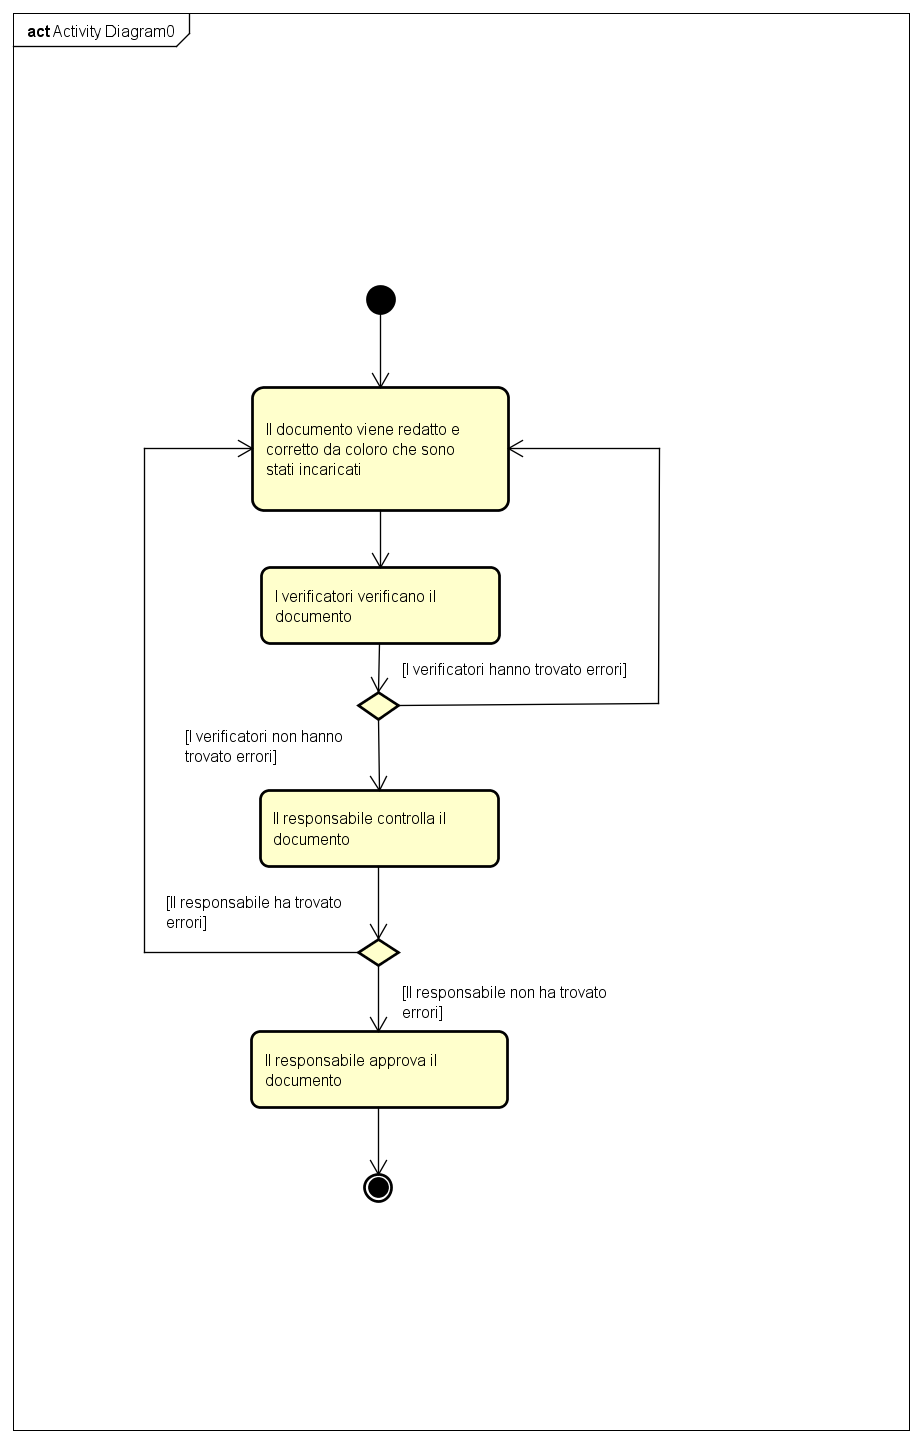
\includegraphics[scale=0.5, width=\textwidth]{sections/img/proceduraFormalizzazioneDocumento.png}
						\caption{Procedura di formalizzazione di un documento}\label{fig:Procedura di formalizzazione di un documento} 
					\end{figure}
		\paragraph{Strumenti}
			\subparagraph{Latex}
				La stesura dei documenti deve essere effettuata utilizzando il linguaggio di markup\g\ \LaTeX\g. È stato scelto questo strumento poiché permette una facile separazione tra formattazione e presentazione. La scelta dell'editor da utilizzare è lasciata libera ai membri del gruppo.
				\subsubparagraph{Template}
					Per poter creare omogeneità tra i documenti, è stato creato un template \LaTeX\g\ nel quale sono state definite tutte le regole tipografiche da applicare al documento. Questo permette di poter scrivere i documenti senza dover tener conto della loro formattazione.
				\subsubparagraph{Comandi personalizzati}
					Sono stati definiti dei comandi \LaTeX\g\ personalizzati al fine di poter rendere più semplice ed immediata l'applicazione delle norme tipografiche. Questi comandi si occupano delle corretta formattazione del testo secondo le norme che sono state definite. La lista dei comandi è presente nella sezione formati.
				\subsubparagraph{Rilevamento errori ortografici}
					Al fine di semplificare l'operazione di individuazione e correzione degli errori ortografici, è stato creato uno script bash \frmfile{OrtographicCheck.sh}.

\subsection{Configurazione}
	\subsubsection{Controllo di versione}
		Il controllo di versione di documenti e file sorgente viene fatto utilizzando il software\g\ Git\g\ e la piattaforma GitHub\g. Ad ogni modifica sostanziale ad un documento o ad un file sorgente impone che a quest'ultimo venga assegnato nuovo numero di versione. \\ Per quanto riguarda le norme di versionamento dei file inerenti alla documentazione si rimanda alla sezione \hyperref[sec:Versionamento dei documenti]{Versionamento dei documenti} del presente documento.
		\paragraph{Richieste di modifica}
			Ogni componente del gruppo può avanzare una richiesta di modifica al \responsabilediprogetto, qualora lo ritenga necessario. Il \responsabilediprogetto\ ha il compito di analizzare tale richiesta e decidere se approvarla o meno. In caso affermativo, deve assegnare il compito di realizzare tale modifica ad un membro del gruppo, in base al ruolo da lui ricoperto in quel momento. Una volta effettuata la modifica questa deve essere sottoposta a verifica e dev'essere fatta mantenendo traccia dello stato precedente. In ogni caso, sia di accettazione della richiesta di modifica, sia in caso di rifiuto, il \responsabilediprogetto\ è tenuto a motivare la scelta.
		\paragraph{Repository}	
			\subparagraph{Struttura del repository}
				I file all'interno del repository\g\ verranno organizzati secondo questa struttura:
				\begin{itemize}
					\item /Documents
					\begin{itemize}
						\item NormeDiProgetto;
						\item StudioDiFattibilità;
						\item AnalisiDeiRequisiti;
						\item PianoDiProgetto;
						\item PianoDiQualifica;
						\item Verbali;
						\item Glossario.
					\end{itemize}
					\item /Source
				\end{itemize}
				La struttura di /Source verrà decisa all'inizio della progettazione architetturale.
			\subparagraph{Commit}
				L'esecuzione di ogni comando commit deve sottostare alle seguenti norme:
				\begin{itemize}
					\item Ad ogni commit è necessario specificare un messaggio nel quale si deve dare una descrizione sintetica e più possibile precisa delle modifiche effettuate;
					\item Le modifiche apportate devono essere complete e testate con successo;
					\item È vietato l'utilizzo del comando \texttt{git add *} prima di un comando commit per evitare di includere nel repository\g\ file nascosti, temporanei o non voluti;
					\item È consigliato specificare il riassunto delle modifiche apportate ad ogni commit tramite il comando \texttt{git commit} rispetto al comando \texttt{git commit -m}, dove il messaggio deve essere scritto inline tra virgolette.
				\end{itemize}
			\subparagraph{Visibilità del repository}
				Per la condivisione e il versionamento dei configuration item è stato creato un repository\g\ privato su GitHub\g, raggiungibile all'indirizzo \url{https://github.com/mzanella/Leaf}. L'accesso è consentito solo ai membri del gruppo.	
			\subparagraph{File}	
				\subsubparagraph{Nomi dei file}
					I nomi dei file interni al repository\g\ devono sottostare alle seguenti norme:
					\begin{itemize}
						\item Devono contenere solo lettere, numeri, il carattere `\_', il segno meno ed il punto;
						\item Devono avere lunghezza minima di tre caratteri;
						\item Devono identificare in modo non ambiguo i file;
						\item Devono riportare le informazioni dal generale al particolare;
						\item Devono, nel caso contengano date, rispettare il formato YYYY-MM-DD.
					\end{itemize}
					È consigliato invece:
					\begin{itemize}
						\item Utilizzare la notazione CamelCase\g, invece di caratteri `\_' e `-' qualora il nome di un file fosse composto da più parole;
						\item Utilizzare nomi né troppo lunghi, né troppo corti, indicativamente tra i 10 e i 25 caratteri, estensione compresa;
						\item Specificare, quando possibile, l'estensione del file.
					\end{itemize}
				\subsubparagraph{Codifica dei file}
					I file contenenti codice oppure documentazione dovranno utilizzare la codifica UTF-8 senza BOM\g.
\newpage
	\subsubsection{Attività}
		\paragraph{Procedure}
			\subparagraph{Procedura di richiesta di modifica}
				Il membro del gruppo che vuole effettuare una modifica deve presentare una richiesta formale al \responsabilediprogetto. La richiesta deve avere i seguenti campi:
				\begin{enumerate}
					\item Autore: contiene nome, cognome e ruolo del richiedente della modifica;
					\item Documento: contiene il nome del documento di cui si ritiene andrebbe fatta tale modifica;
					\item Urgenza: indica una misura di quanto il richiedente ritiene necessario fare una modifica, può assumere solamente tali valori:
						\begin{enumerate}
							\item ``Alta'': in questo caso si ritiene che la modifica da fare sia importante, con pesanti conseguenza nell'organizzazione dello svolgimento delle attività future o che possa in qualche modo compromettere l'organizzazione delle attività future;
							\item ``Media'': in questo caso il richiedente considera la modifica importante, ma non comporta forti conseguenza nell'organizzazione generale delle attività, ma può influenzare lo svolgimento di alcune di queste;
							\item ``Bassa'': in questo caso la modifica proposta di modifica è di importanza secondaria, un suggerimento nell'effettuare alcune attività oppure che non influisce, o il suo peso è poco rilevante, nello svolgimento delle attività.
						\end{enumerate}
					\item Descrizione: una descrizione dettagliata e motivata delle modifiche che si vogliono apportare;
					\item Decisione del \responsabilediprogetto. Questo campo va aggiunto successivamente alla decisione del \responsabilediprogetto. Questo campo può assumere due valori:
						\begin{enumerate}
							\item ``Approvata'';
							\item ``Respinta''.
						\end{enumerate}
					In caso lo ritenga necessario, il \responsabilediprogetto\ può aggiungere a questo campo la motivazione per cui ha approvato o meno la modifica.
				\end{enumerate}
				\newpage
				\begin{figure}[H]
					\centering
					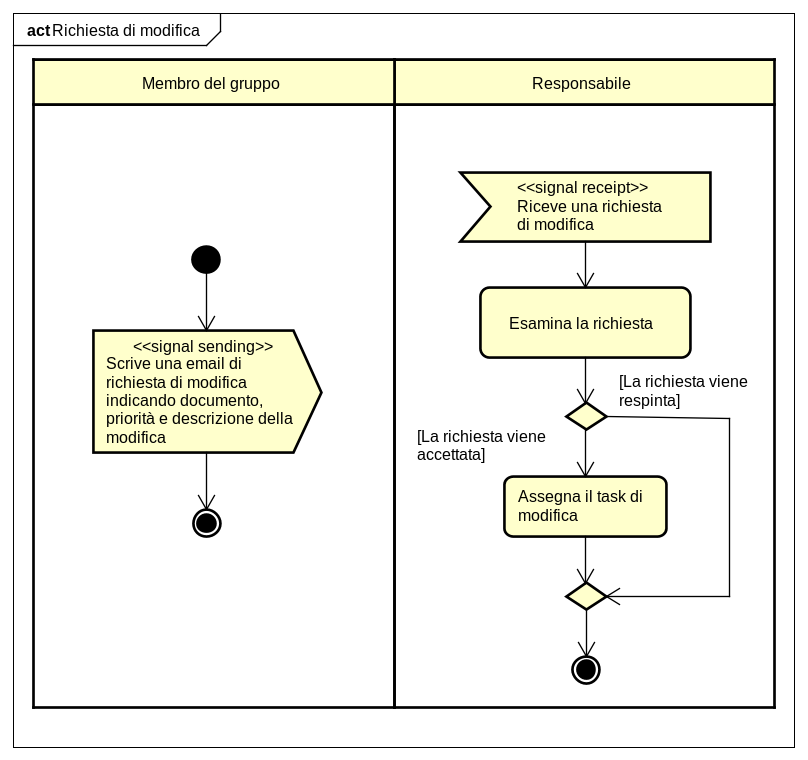
\includegraphics[scale=0.5, width=\textwidth]{sections/img/proceduraRichiestaModifica.png}
					\caption{Procedura di richiesta modifica di un documento}\label{fig:Procedura di richiesta modifica di un documento} 
				\end{figure}
			\subparagraph{Aggiornamento del repository}
				Per l'aggiornamento del repository\g\ è prevista la seguente procedura:
				\begin{itemize}
					\item Dare il comando \texttt{git pull}. Nel caso in cui si verifichino dei conflitti:
						\begin{itemize}
							\item Dare il comando \texttt{git stash} per accantonare momentaneamente le modifiche apportate;
							\item Dare il comando \texttt{git pull};
							\item Dare il comando \texttt{git stash apply} per ripristinare le modifiche.
						\end{itemize}
					In questo modo il repository\g\ risulta aggiornato rispetto il repository\g\ remoto;
					\item Dare il comando \texttt{git add NomeDelFile}, dove al posto di ``NomeDelFile'' si deve mettere il nome del file, o lista di nomi dei file, sul quale sono state effettuate delle modifiche;
					\item Dare il comando \texttt{git commit}, e successivamente specificare sinteticamente il riassunto delle modifiche effettuate;
					\item Dare il comando \texttt{git push}.
				\end{itemize}
				\begin{figure}[H]
					\centering
					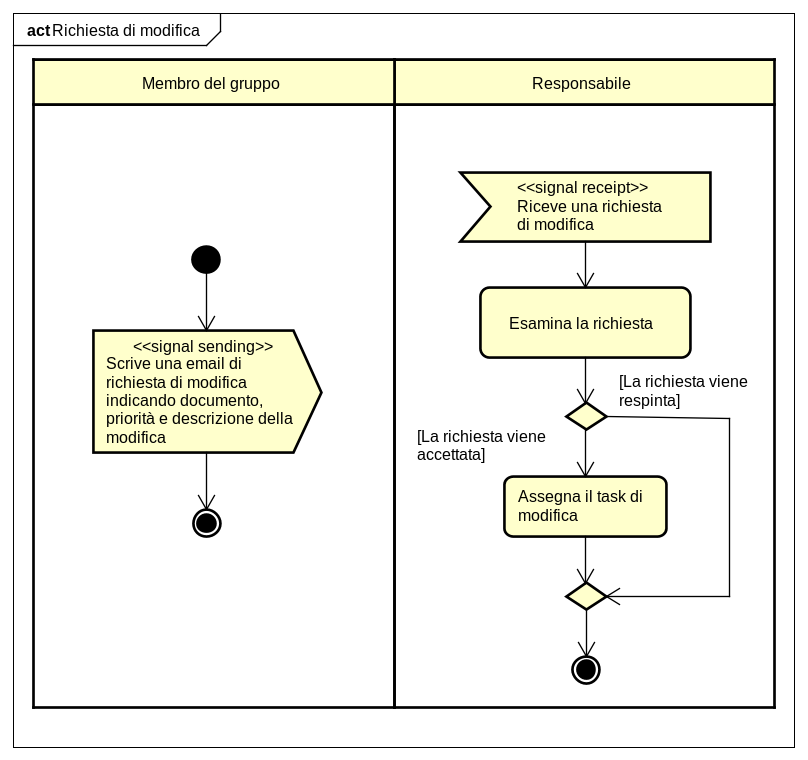
\includegraphics[scale=0.5, width=\textwidth]{sections/img/proceduraRichiestaModifica.png}
					\caption{Procedura di aggiornamento del repository}\label{fig:Procedura di aggiornamento del repository} 
				\end{figure}	
		\paragraph{Strumenti}
			Lo strumento utilizzato per il versionamento di documenti e file sorgenti è Git\g. Nonostante siano presenti varie alternative, come Mercurial, Subversion e Bazaar, è stato scelto Git\g\ in quanto soddisfa appieno le necessità di versionamento dei file per questo progetto e, inoltre, permette di versionare i file localmente, senza bisogno di una connessione internet attiva. Come servizio di hosting per il repository\g\ è stato scelto, invece, GitHub\g. Entrambe le scelte sono state fatte anche perché più membri del gruppo avevano già avuto la possibilità di lavorare con tali servizi.
	
	
\subsection{Verifica}
	\subsubsection{Verifica dei documenti}
		Il \responsabilediprogetto\ ha il compito di dare inizio alla fase\g\ di verifica, assegnando i compiti ai \verificatori. Quest'ultimi, devono effettuare un'accurata verifica delle seguenti regole:
		\begin{itemize}
			\item Deve essere utilizzata una sintassi corretta e il più possibile semplice;
			\item Devono essere utilizzati periodi brevi;
			\item La struttura del documento deve essere semplice e intuitiva;
			\item Devono essere rispettate le  \hyperref[sec:Norme tipografiche]{norme tipografiche};
			\item Devono essere rispettate le \hyperref[sec:Glossario]{regole riguardanti il glossario}.
		\end{itemize}
		Durante l'intera attività di verifica i \verificatori\ dovranno utilizzare lo strumento del diario delle modifiche in modo tale da concentrare la loro attenzione sulle modifiche effettuate ad un documento e tenere traccia degli errori più comuni commessi nel redigere i documenti.
		\paragraph{Sintassi}
			I \verificatori\ hanno il compito di identificare errori sintattici nei documenti. Ciò può essere fatto con l'ausilio di strumenti automatici, ma ogni documento deve essere sempre sottoposto a walkthrough in modo tale da individuare errori che non sono stati in grado di evidenziare. Inoltre hanno il compito di inserire nel \glossario\ tutte quelle parole che possono essere fonte di ambiguità.
		\paragraph{Periodi}
			I \verificatori\ hanno il compito di calcolare l'indice Gulpease\g\ di ogni documento utilizzando lo strumento automatico preposto (vedi sezione \hyperref[sec:Strumenti]{Strumenti}). Qualora non si ottenga un risultato soddisfacente il \verificatore\ deve applicare la tecnica walkthrough con l'obiettivo di individuare periodi troppo lunghi, che possono essere di difficile comprensione o leggibilità.
		\paragraph{Struttura del documento}
			I \verificatori\ devono verificare che la struttura di ogni documento rispetti i contenuti del documento stesso.
	\subsubsection{Diagrammi UML}
		I \verificatori\ devono controllare tutti i diagrammi UML\g\ prodotti, sia che venga rispettato lo standard UML\g, sia che siano corretti semanticamente. I diagrammi utilizzati finora sono solamente i diagrammi dei casi d'uso.
			\paragraph{Diagrammi dei casi d'uso}
				Le verifiche che devono essere effettuate ai diagrammi dei casi d'uso, innanzitutto, devono riguardare il rispetto dello standard UML\g, soprattutto riguardanti inclusioni, generalizzazioni e estensioni. Successivamente si deve verificare che la semantica del diagramma sia corretta, ovvero che il diagramma rappresenti effettivamente ciò che si vorrebbe descrivere e modellare. Per quest'ultimo punto bisogna porre particolare attenzione sull'identificazione degli attori. Per questo motivo è prevista una \hyperref[par:Procedura di verifica degli attori dei diagrammi UML]{procedura di verifica degli attori dei diagrammi UML} in questo documento.\\ 
	\subsubsection{Issue tracking}
		L'issue\g\ tracking è un'attività di supporto per i \verificatori\ ai quali permette di tenere traccia potenziali errori, segnalandoli al \responsabilediprogetto. Lo strumento scelto per la gestione di questa attività è GitHub(vedi sezione \hyperref[par:IssueTrk GitHub]{Strumenti}). Questo strumento è utile anche al \responsabilediprogetto\ per assegnare i compiti di correzione degli errori. 
		\paragraph{Sintassi di una label}
			Le label sono delle etichette che è possibile associare ad ogni issue\g. Ogni etichetta rappresenta lo stato nel quale si trova la issue. Le uniche etichette che sono accettate sono le seguenti:
			\begin{itemize}
				\item \textbf{Request}: rappresenta la richiesta di una issue\g;
				\item \textbf{Question}: identifica una issue\g\ nella quale si sta discutendo per risolvere il problema;
				\item \textbf{ToDo}: identifica una issue\g\ per la quale è stata trovata la soluzione ma questa deve ancora essere applicata;
				\item \textbf{Working}: identifica una issue\g\ alla quale un membro del gruppo sta lavorando per applicare la soluzione;
				\item \textbf{Rejected}: identifica una issue\g\ che non è stata accettata poiché risulta essere futile o dannosa;
				\item \textbf{Done}: identifica una issue\g\ che è stata completata.
			\end{itemize}				
		\paragraph{Sintassi di una Issue}
			Ogni issue\g\ avrà un nome che dovrà seguire la seguente notazione: \begin{center}\textbf{[D]:[S]}\end{center} dove:
				\begin{itemize} 
					\item \textbf{D} rappresenta la sigla del documento di interesse;
					\item \textbf{S} rappresenta la sintesi della descrizione del problema.
				\end{itemize}
				Segue, poi, la descrizione della issue\g. Questa dovrà obbligatoriamente contenere:
			\begin{itemize} 
				\item dove si trova il problema. Questo va specificato tramite sezione e, possibilmente, numero di riga dove inizia il problema;
				\item una descrizione dettagliata del problema che deve comprendere:
				\begin{itemize}
					\item tutte gli errori associati al problema. Questi devono essere riportati nella forma di checkbox. Per fare ciò è necessario premettere alla descrizione di ogni errore i caratteri \texttt{ - [ ]}. Questo permette di facilitare il tracciamento dello stato di avanzamento della issue\g.
					\item una eventuale porzione di codice che potrebbe essere causa del problema. Per fare ciò è consigliabile utilizzare il comando: \begin{center} \texttt {\`{}\`{}\`{}nomelinguaggio\\ codice da riportare\\ \`{}\`{}\`{}} .\end{center} Sostituendo ``nomelinguaggio'' al nome del linguaggio di programmazione utilizzato, si potrà vedere la porzione di codice evidenziata secondo la sintassi del linguaggio stesso, facilitandone la lettura.
				\end{itemize}
				\item la motivazione per cui si è ritenuto necessario sollevare una issue\g.
			\end{itemize}
		
		\paragraph{Resoconto attività di verifica sui documenti}
			\subparagraph{Attività manuale di verifica}		
			Ogni attività manuale di verifica sui documenti deve essere accompagnata da un resoconto. Il resoconto deve contenere il numero di occorrenze riscontrate durante la verifica per ognuna delle seguenti voci:
			\begin{itemize}
				\item periodi troppo lunghi o complessi;
				\item parole non appropriate;
				\item incongruenze;
				\item errori concettuali;
				\item violazioni di quanto stabilito nelle norme tipografiche.		
			\end{itemize}
			Al fine di rendere più veloce e chiara l'analisi di queste voci, è consigliabile che questi dati vengano rappresentati in forma tabellare.\\
			Inoltre, deve essere sempre presente una tabella contenente il numero di occorrenze riscontrate durante la verifica per ognuna delle seguenti voci:
				\begin{itemize}
					\item termini candidati ad essere aggiunti al \glossario;
					\item termini aggiunti al \glossario.
				\end{itemize}
				\subparagraph{Attività automatica di verifica}
				Ogni attività automatica di verifica sui documenti deve essere accompagnata da un resoconto. Il resoconto deve contenere il numero di occorrenze riscontrate durante la verifica per ognuna delle seguenti voci:
				\begin{itemize}
				\item errori ortografici;
				\item utilizzo errato \LaTeX\g;	
				\end{itemize}
			
			Inoltre, devono essere riportarti gli indici Gulpease calcolati per ognuno dei documenti sui quali è stata effettuata attività di verifica.
			
	\subsubsection{Attività}
		\paragraph{Procedure}	
			\subparagraph{Tecniche di analisi}
				Per poter verificare la qualità del prodotto\g\ è stato scelto di applicare delle tecniche di analisi sui documenti e sul codice. 
				\subsubparagraph{Analisi statica} 
					Per analisi statica si intende la valutazione di un sistema basata su struttura, contenuto e documentazione senza che questo venga eseguito. Questa tecnica è applicabile sia al codice, che alla documentazione stessa. L'analisi statica può avvenire con due modalità:
					\begin{itemize}
						\item \textbf{Walkthrough}: questa tecnica dev'essere applicata quando non si sa che errori o problematiche si stanno cercando. La tecnica consiste nel leggere il codice sorgente o il documento da cima in fondo per trovare anomalie  di qualsiasi tipo;
						\item \textbf{Inspection}: questa tecnica dev'essere applicata quando si ha idea della problematica che si sta cercando e consiste in una lettura mirata del documento/codice, sulla base di una lista degli errori precedentemente stilata.
					\end{itemize}
					La tecnica walkthrough è molto onerosa e deve essere utilizzata soprattutto nelle prime fasi del progetto, quando non è già presente una lista degli errori comuni, oppure non si è ancora sufficientemente preparati riguardo un aspetto del progetto. Avanzando nelle fasi del progetto sarà utile stilare una lista quanto più possibile completa di errori comuni, in modo tale da evitare la tecnica walkthrough e applicare l'inspection.
				
				\subsubparagraph{Analisi dinamica}
					L'analisi dinamica è una forma di valutazione di un sistema software\g, oppure di qualche suo componente, basato sull'osservazione del suo comportamento durante l'esecuzione. Questa tecnica non è applicabile, quindi, per trovare errori nella documentazione. I test che devono essere implementati devono essere in numero relativamente ridotto e il più possibile di valore dimostrativo.
		
			\subparagraph{Resoconto attività di verifica sui documenti}	
				La stesura dell'attività del resoconto dell'attività di verifica dovrà essere fatta al termine dell'attività di verifica. Il \verificatore\ dovrà riportare il numero di occorrenze per ognuna delle voci definite nella sezione norme. Qualora fossero stati trovati degli errori nelle attività di verifica precedenti, il numero di errori trovati andrà a sommarsi al numero di errori trovati nelle attività precedenti.
				Inoltre, il \verificatore, nel caso in cui dovesse trovare termini mancanti nel glossario, dovrà aggiornare la tabella definita nelle norme che regolano l'attività manuale di verifica.
			
			\subparagraph{Gestione di una issue}
				Qualora i \verificatori\ dovessero riscontrare delle anomalie, la procedura per la segnalazione e gestione del ticketing di una issue\g\ è la seguente:
					\begin{enumerate}
						\item il \verificatore\ che ha riscontrato un'anomalia\g\ dovrà aprire una nuova issue\g\ assegnandole l'etichetta Request;
						\item il \responsabilediprogetto\ dovrà valutare la issue\g\ e decidere se:			\begin{itemize}
							\item la issue\g\ risulta essere futile o dannosa. In questo caso verrà rimossa l'etichetta Request ed assegnata l'etichetta Rejected. La issue\g\ verrà poi chiusa, terminando la procedura.
							\item la issue\g\ risulta essere appropriata. In questo caso verrà rimossa l'etichetta Request ed assegnata l'etichetta Question. 
						\end{itemize}
						\item i membri del gruppo dovranno discutere e proporre nuove idee al fine di risolvere la issue\g. Questa discussione non dovrà protrarsi per più di tre giorni. Qualora non si dovesse essere trovata una soluzione ottimale, il \responsabilediprogetto\ dovrà decidere quale sia la soluzione migliore.
						\item il \responsabilediprogetto, trovata la soluzione da applicare,  assegnerà, al membro del gruppo da lui ritenuto opportuno, un ticket\g. L'assegnatario del ticket\g\ è la persona incaricata all'applicazione della soluzione relativa alla issue\g. Inoltre, il \responsabilediprogetto\ dovrà rimuovere dalla issue\g\ l'etichetta Question ed assegnare l'etichetta ToDo.
						\item quando l'incaricato inizierà a lavorare sulla issue\g\ rimuoverà l'etichetta ToDo ed assegnerà l'etichetta Working. Ad ogni nuovo commit, l'incaricato dovrà riferire, nel messaggio del commit stesso, la issue\g\ sulla quale sta lavorando. Questo permetterà di tener traccia delle modifiche effettuate per risolvere la issue\g.
						\item una volta che l'incaricato avrà terminato le modifiche, queste dovranno essere caricate nel repository\g\ e l'etichetta della issue\g\ dovrà essere modificata da Working a Done. Dopo che sono state svolte queste operazioni, la issue\g\ verrà chiusa.
					\end{enumerate}
\newpage
				\begin{figure}[H]
					\centering
					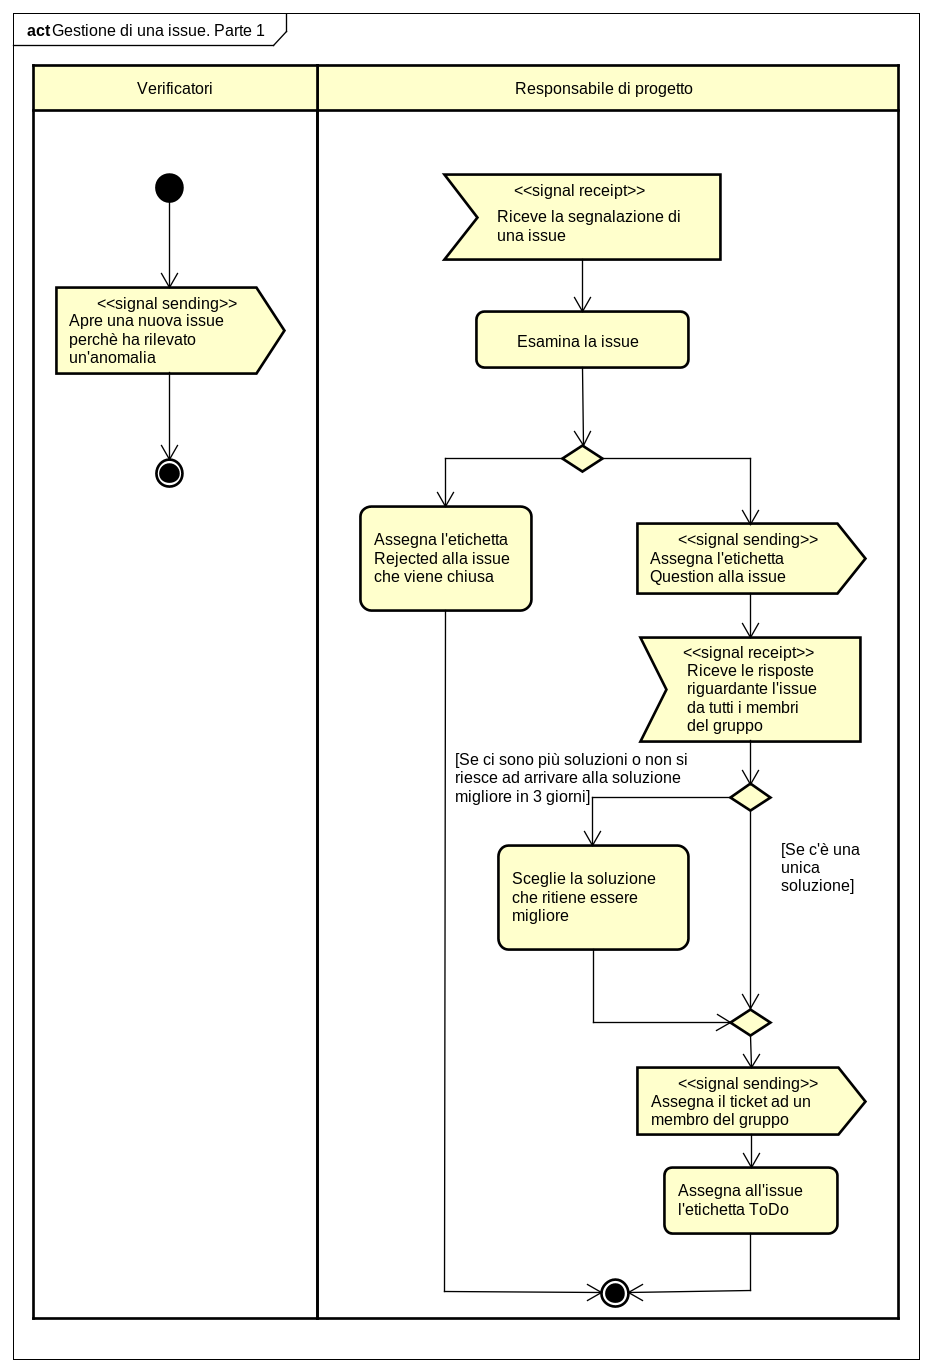
\includegraphics[scale= 0.75, width=\textwidth]{sections/img/gestioneIssueP1.png}
					\caption{Procedura di gestione di una issue. Parte 1}\label{fig:Procedura di gestione di una issue parte 1} 
				\end{figure}

				\begin{figure}[H]
					\centering
					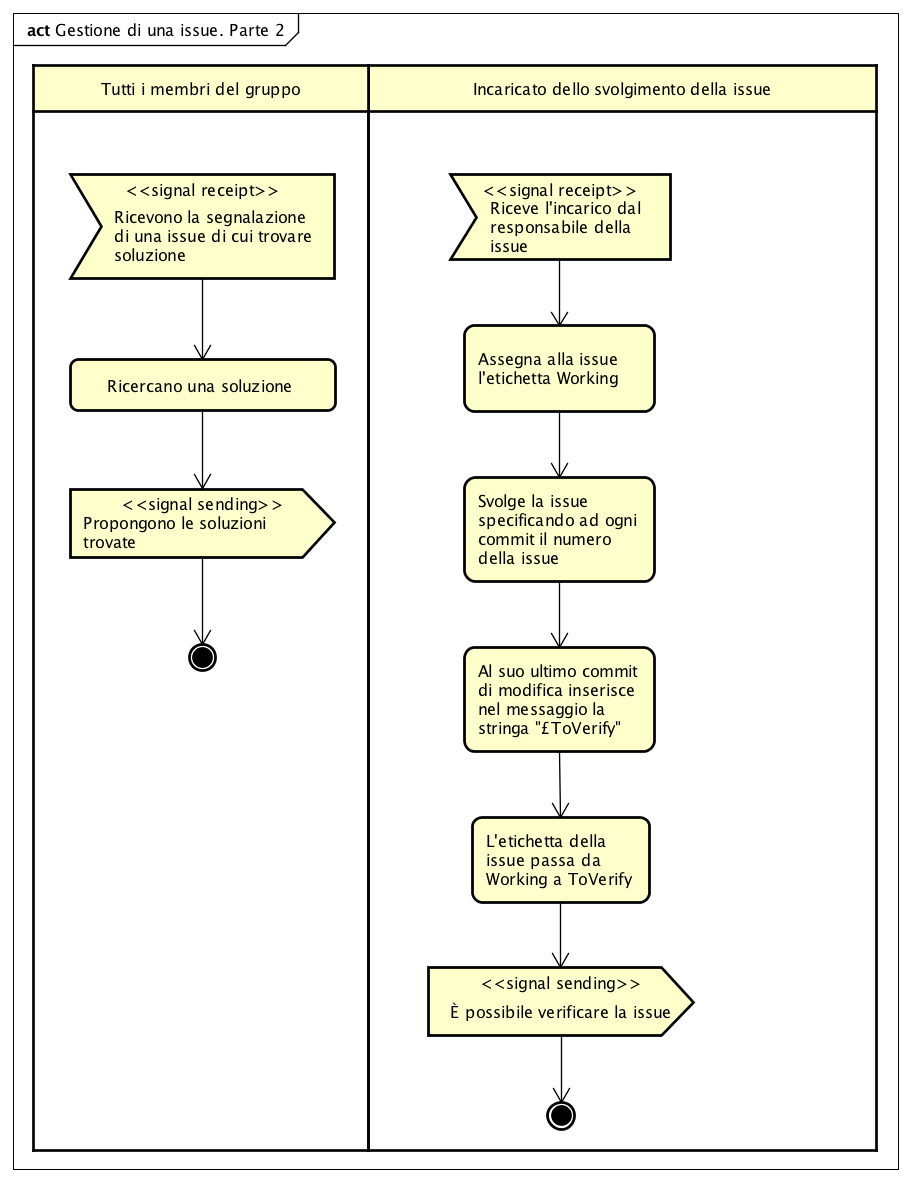
\includegraphics[scale= 0.75, width=\textwidth]{sections/img/gestioneIssueP2.png}
					\caption{Procedura di gestione di una issue. Parte 2}\label{fig:Procedura di gestione di una issue parte 2} 
				\end{figure}

		\subparagraph{Procedura di verifica attori dei diagrammi UML}\label{par:Procedura di verifica degli attori dei diagrammi UML}
			Per identificare un attore può risultare utile seguire la seguente procedura:
			\begin{enumerate}
				\item Per prima cosa è utile chiedersi se ciò che vogliamo rappresentare come attore è una persona che interagisce col sistema. In caso affermativo è giusto rappresentarlo come attore, in caso negativo si deve andare al passo 2;
				\item Se ciò che vogliamo rappresentare come attore non è una persona che interagisce col sistema bisogna chiedersi se questa ``cosa'' può cambiare insieme al design del sistema. In caso affermativo probabilmente ciò che vogliamo rappresentare non è un attore ma una parte del sistema stesso. In caso negativo, invece, è con buona probabilità un attore.
			\end{enumerate}
			\begin{figure}[H]
				\centering
				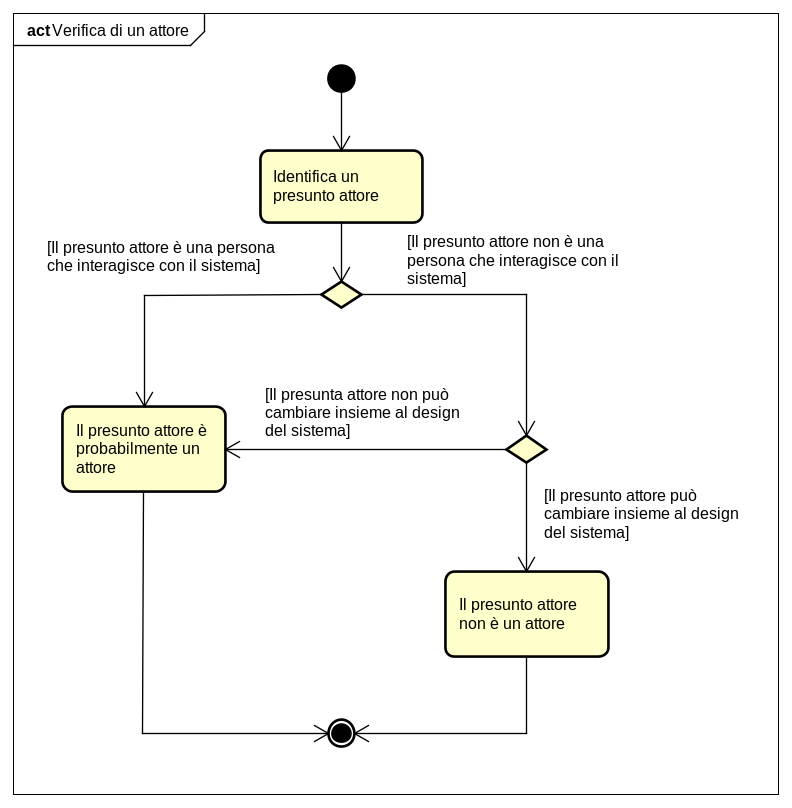
\includegraphics[scale=0.5, width=\textwidth]{sections/img/proceduraVerificaAttori.png}
				\caption{Procedura di verifica di un attore}\label{fig:Procedura di verifica di un attore} 
			\end{figure}
\newpage
		\paragraph{Strumenti} \label{sec:Strumenti}
			\subparagraph{Strumento per l'issue tracking} \label{par:IssueTrk GitHub}
				Lo strumento scelto per fare il tracking delle issue\g\ è il servizio Issues messo a disposizione da GitHub\g. 
	
\subsection{Processo di validazione}
		Il processo di validazione ha l'obbiettivo di verificare che: 
		\begin{itemize}
			\item il prodotto finale sia conforme a quanto è stato pianificato;
			\item il prodotto finale sia abile nell'isolare e minimizzare gli effetti degli errori.
		\end{itemize}

		\subsubsection{Responsabilità}
			Di seguito si elencano le rispettive responsabilità per la validazione del prodotto: 
			\begin{itemize}
				\item i \verificatori\ hanno il compito di eseguire con attenzione i test, tracciandone i risultati che andranno poi valutati;
				\item il \responsabilediprogetto\ revisiona i risultati dei test e decide se accettarli o ripeterli. Ha inoltre il compito di informare il committente dell'esecuzione e risultato dei test, fornendo indicazioni sulla possibilità di eseguirli in modo indipendente.
			\end{itemize}
		\subsubsection{Attività}
			\paragraph{Procedure}
				\subparagraph{Validazione}
					I passi per eseguire l'attività di validazione sono i seguenti:
					\begin{enumerate}
						\item i \verificatori\ eseguono manualmente i test sul prodotto finale, tracciando accuratamente i risultati ottenuti;
						\item il \responsabilediprogetto\ di progetto analizza i risultati e decide se:
							\begin{enumerate}
							 	\item accettarli;
							 	\item chiedere una ripetizione di alcuni o tutti i test, eventualmente con verificatori diversi.
							 \end{enumerate}  
						\item una volta accettati i test, il \responsabilediprogetto\ consegna i risultati al proponente, informandolo sulle modalità di esecuzione indipendente della validazione.
					\end{enumerate}
\end{document}
